\chapter{Classical optimisation scheme for FEM model}
%The way to build the optimization chain with metamodelisation Paper1

 \subsubsection{Sensitivity analysis}
    

  The global sensitivity analysis for the involved shape parameters was performed using the Variance-based method which comes from Hoeffding-Sobol decomposition. This method is based on decomposing the variance of a function to its variance associated with the parameters and the interaction between the parameters. Hence, higher the variance in output of a function induced by a parameter infers higher sensitivity. The method is applied through Monte-Carlo based estimation defined by latin hypercube sampling for efficiency. In effect, to evaluate the global behaviour and to increase the accuracy for the given Monte-Carlo based estimation on the presumed asymptotic case demands a large computation of design points, which is simply impossible to converge with a reasonable time given the computation cost to evaluate the stability criteria. Hence, a surrogate model based on Gaussian process regression was used, detailed in section . The stability criteria given by the surrogate model is defined as $\hat C_s$, where $ C_s \approx \hat C_s$.\\ 

To understand the effect of the shape parameters on the stability criteria, the first-order and the total-order sensitivity indices are computed. The first-order indices define the contribution of a given parameter to the change in unconditional variance $V(\hat C_s)$, while the total-order indices add to it the contribution of all the higher-order interactions on the given parameter. The general expression for the first-order index $S_i$ and the total-order index $S_{Ti}$  can be given as 

\begin{equation}
S_i = \dfrac{V_{X_i}(E_{X_{\sim i}}(\hat C_s|X_i))}{V(\hat C_s)}
\end{equation}

\begin{equation}
S_{Ti} = 1-\dfrac{V_{X_{\sim i}}(E_{X_i}(\hat C_s|X_{\sim i}))}{V(\hat C_s)}
\end{equation}

where ${V_{X_i}(E_{X_{\sim i}}(\hat C_s|X_i))}$ is the variance of the conditional expectation on the function of the stability criteria $\hat C_s$ evaluated by conditioning the parameter $X_i$ for several values across the bounded design space and similarly, ${V_{X_{\sim i}}(E_{X_i}(\hat C_s|X_{\sim i}))}$ is the variance of the conditional expectation obtained by conditioning all parameters except for $X_i$. \\

The described probability measures are estimated based on the estimators proposed in . The Monte-Carlo based estimation for the given estimators require two matrices $Y_A$ and $Y_B$ of equal size with rows and columns representing the design points and the parameters respectively. To evaluate the first order index of the $i$th parameter, all the parameters of $Y_B$ are unchanged except for the $i$th parameter ($i$th column of the matrix) which is replaced by the $i$th parameter of $Y_A$ to obtain the matrix $Y_{Bi}$. Similarly, to evaluate the total-order index of the $i$th parameter, all the parameters of $Y_B$ are changed with the parameters of $Y_A$ except for the $i$th parameter to obtain the matrix $Y_{Bti}$. Hence, the matrices $Y_{Bi}$ and $Y_{Bti}$ represent the conditioning of the parameters with respect to the matrix $Y_A$, which in a sense is used to evaluate the conditional probability terms and also to describe the effective unconditional variance, as given by the estimators. For $n$ parameters and $p$ design points where the parameters are to be conditioned, it requires an estimation of $(n+1)p$ design points to evaluate the first order index or the total order index of all the parameters.\\

The sensitivity analysis was performed on seven shape parameters as in table \ref{tab:Parameters_range} describing the complete geometry of the considered model. The value of $p$ as described in section \ref{sensitivity_analysis} is chosen to be 1500 and hence evaluating a total of 24000 design points with meta-model to evaluate the first-order and the total-order indices. The evaluation was repeated for different sample sets to check for convergence, which is seen to be not difficult with the chosen $p$ value and with an estimated standard error for the indices of no more than 0.02.\\

\begin{figure}
    \centering
    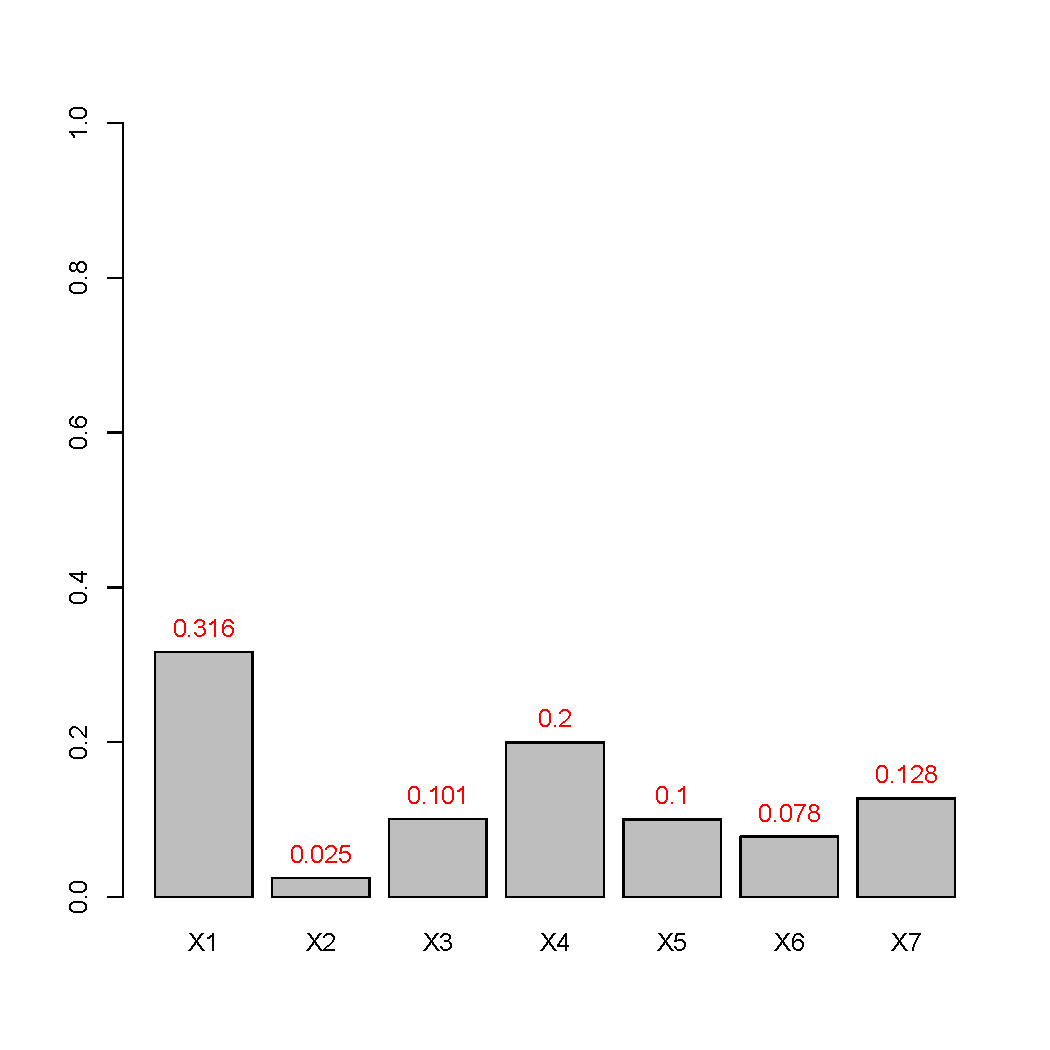
\includegraphics[scale=0.53]{Chapter2/Pictures/first_sobol.pdf}
    \caption{First-order Sobol indices}
\end{figure}

\begin{figure}
    \centering
    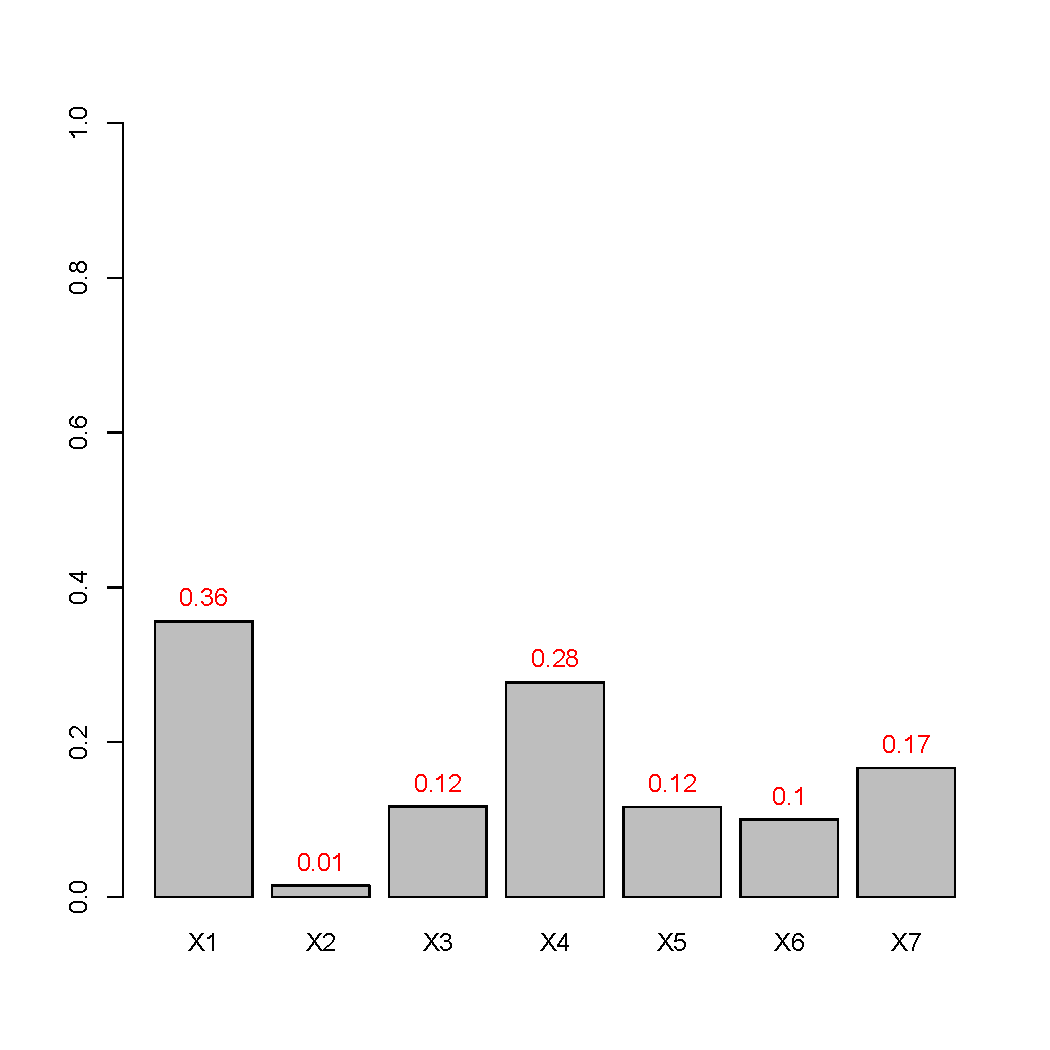
\includegraphics[scale=0.53]{Chapter2/Pictures/total_sobol.pdf}
    \caption{Total-order Sobol indices}
\end{figure}

The description of the parameters are as in  %\ref{tab:Parameters_range}.
\iffalse
\sout{follows, X1 - Thickness of the disc, X2 - Outer radius of the disc, X3 - Inner radius of the disc, X4 - Thickness of the pad, X5 - Inner radius of the pad, X6 - Outer radius of the pad and X7 - Angle of the pad.} 
\fi

As it can be seen, the first-order indices show relatively high values for the parameters X1 - thickness of the disc and X4 - thickness of the pad. The total-order indices also increase relatively for the two parameters. But the global variance of the stability criteria can be largely attributed to independent effects from the parameters rather than interaction between them. \\

Further, the results are also shown with closed second-order indices, combining the independent effects and the interaction between any two parameters.

\begin{figure}
    \centering
    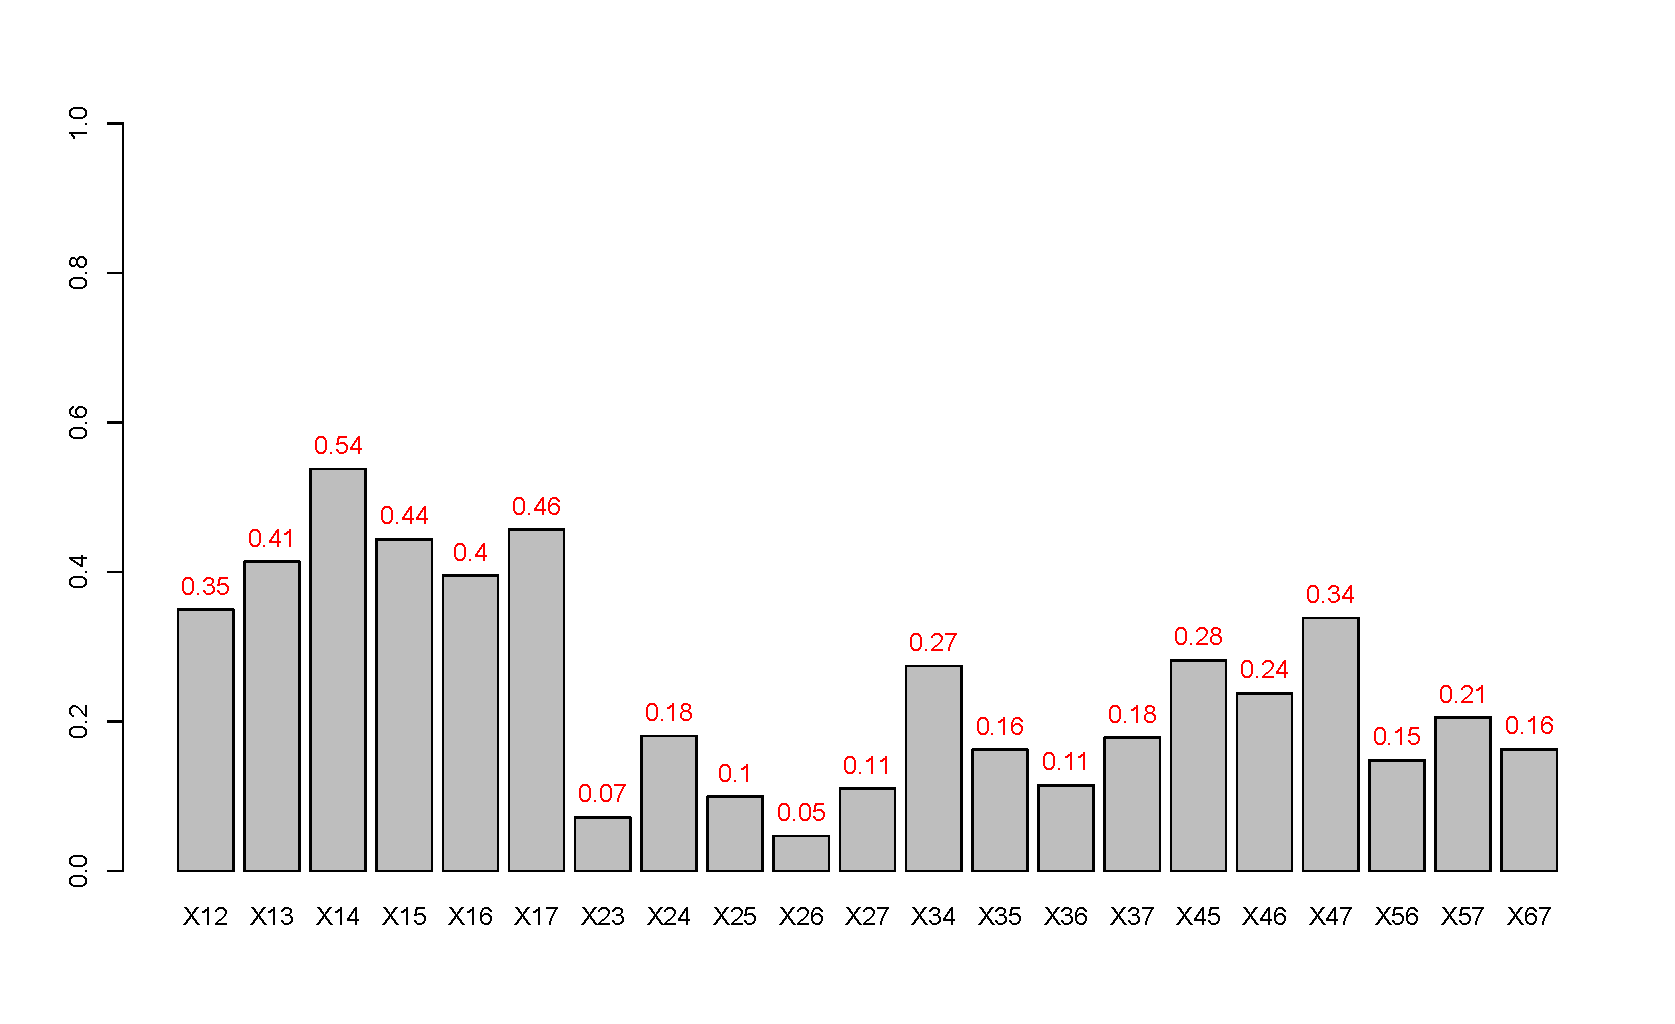
\includegraphics[scale=0.53]{Chapter2/Pictures/second_order_sobol.pdf}
    \caption{Closed second-order Sobol indices}
\end{figure}
